\usepackage{float}

\usepackage{tikz}
\usetikzlibrary{positioning}
\definecolor{processcolor}{cmyk}{0.96,0,0,0}


\newcommand{\markovchain}{
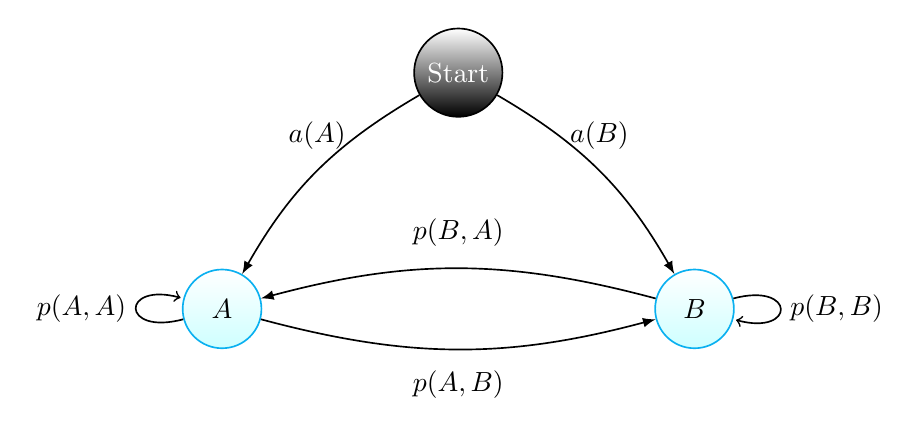
\begin{tikzpicture}[-latex, auto, node distance = 3cm and 3cm, on grid,
                    semithick,
                    state/.style = {circle,
                                    top color = white,
                                    bottom color = processcolor!20,
                                    draw,
                                    processcolor,
                                    text = black,
                                    minimum width = 1 cm},
                    initial/.style = {circle,
                                      top color = white,
                                      bottom color = black,
                                      draw,
                                      black,
                                      text = white,
                                      minimum width = 1 cm}]

\node[initial] (S) {Start};
\node[state] (A) [below left  = of S] {$A$};
\node[state] (B) [below right = of S] {$B$};

\path (S) edge [bend left = -15] node[above = 0.15 cm] {$a(A)$} (A);
\path (S) edge [bend right = -15] node[above = 0.15 cm] {$a(B)$} (B);

\path (A) edge [loop left] node[left] {$p(A, A)$} (A);
\path (A) edge [bend right = 15] node[below = 0.15 cm] {$p(A, B)$} (B);
\path (B) edge [loop right] node[right] {$p(B, B)$} (B);
\path (B) edge [bend left = -15] node[above = 0.15 cm] {$p(B, A)$} (A);

\end{tikzpicture}
}


\newcommand{\hiddenmarkovmodel}{
\begin{tikzpicture}[-latex, auto, node distance = 3cm and 3cm, on grid,
                    semithick,
                    observe/.style = {rectangle,
                                      top color = white,
                                      bottom color = green!20,
                                      draw,
                                      green,
                                      text = black,
                                      minimum width = 1 cm},
                    state/.style = {circle,
                                    top color = white,
                                    bottom color = processcolor!20,
                                    draw,
                                    processcolor,
                                    text = black,
                                    minimum width = 1 cm},
                    initial/.style = {circle,
                                      top color = white,
                                      bottom color = black,
                                      draw,
                                      black,
                                      text = white,
                                      minimum width = 1 cm}]

\node[initial] (I) {Start};
\node[state] (S1) [below left  = of S] {$S_1$};
\node[state] (S2) [below right = of S] {$S_2$};
\node[observe] (v1) [below = of A] {$v_1$};
\node[observe] (v2) [below = of B] {$v_2$};

\path (I) edge [bend left = -15] node[above = 0.15 cm] {$\pi_1$} (S1);
\path (I) edge [bend right = -15] node[above = 0.15 cm] {$\pi_2$} (S2);

\path (S1) edge [loop left] node[left] {$a_{11}$} (S1);
\path (S1) edge [bend right = 15] node[above = 0.15 cm] {$a_{12}$} (S2);
\path (S2) edge [loop right] node[right] {$a_{22}$} (S2);
\path (S2) edge [bend left = -15] node[above = 0.15 cm] {$a_{21}$} (S1);

\path (S1) edge [bend left = -15] node[left = 0.15 cm] {$b_1(1)$} (v1);
\path (S2) edge [bend left = 15] node[right = 0.15 cm] {$b_2(2)$} (v2);
\path (S1) edge [bend left = -15] node[left = 0.1 cm] {$b_1(2)$} (v2);
\path (S2) edge [bend left = 15] node[right = 0.1 cm] {$b_2(1)$} (v1);

\end{tikzpicture}
}